\documentclass[twocolumn]{article}
\usepackage{graphicx}
\usepackage{fullpage}
\usepackage{amssymb}
\usepackage{amsmath}
\usepackage{listings}
\usepackage{color}

\definecolor{dkgreen}{rgb}{0,0.6,0}
\definecolor{gray}{rgb}{0.5,0.5,0.5}
\definecolor{mauve}{rgb}{0.58,0,0.82}

\lstset{frame=tb,
  language=C,
  aboveskip=3mm,
  belowskip=3mm,
  showstringspaces=false,
  columns=flexible,
  basicstyle={\small\ttfamily},
  numberstyle=\tiny\color{gray},
  keywordstyle=\color{mauve},
  commentstyle=\color{dkgreen},
  stringstyle=\color{green},
  breaklines=true,
  breakatwhitespace=true,
  tabsize=3
}

\title{\textbf{The exponential function}}
\author{Sofie Jastrup Lanng}
\date{\today}

\begin{document}
\maketitle

\section{The exponential function}
The real exponential function $\exp(x): \mathbb{R}\rightarrow\mathbb{R}$ is formally defined from the power series
\begin{equation}\label{eq:power}
	\exp(x) = \sum_{k=0}^\infty \frac{x^k}{k!} \;.
\end{equation}
This convergence radius of this series is infinite, and hence the exponential function may be extended to the complex numbers $\mathbb{C}$.

\section{A numerical approximation}
In this exercise we use the approximation scheme as seen in the following code snippet

\begin{lstlisting}
#include<math.h>
double myExp(double val){
  if( val < 0    ) {
    double result  =  1.0 / myExp( -val   );
    return result;
  }
  if( val > 1./8 ) {
    double result  =  pow( myExp( val / 2 ), 2 );
    return result;
  }
  double result =
		1 + val*( 1 + val/2*( 1 + val/3*( 1 + val/4*(1 + val/5*( 1 + val/6*( 1 + val/7*( 1 + val/8*( 1 + val/9*( 1 + val/10) ) ) ) ) ) ) ) );
  return result;
}

\end{lstlisting}
In this implementation input values, the query points are specified by the double valued parameter val.
We begin by checking for negative inputs, in which case we should recursively return the inverse of the function value,
of the corresponding positive input value, i.e. $\exp \left( -\text{val} \right)^{-1}$. This implementation, being the taylor series around zero,
will be most accurate for small values, so we should hence next check for the size of the input value. Squaring the exponential function, due to the
nature of exponents, will be the same as doubling the input value, hence the division by two. This ensures the input value can be made arbitrarily
small. Thus, we recursively do this untill the input value is a number of value smaller than $\frac18$. The final computation of the taylor serises
is then performed. Instead of using exponents, we simply multiply the value onto it self and arbitrary number of times. The time complexity of this
operation is low, so it is very fast. It has the added advantage that we are not computing factorials, that is, very large numbers, that will conflict
with our precision very quikly. Hence the computer will not be forced to add up numbers of different orders of magnitude, and we retain precision.

\section{Figures}
Here is an illustration of the numerical implementation that was described above in figure~(\ref{fig:pyxplot})
shows the "pdf" terminal of Pyxplot.


\begin{figure}[h]
	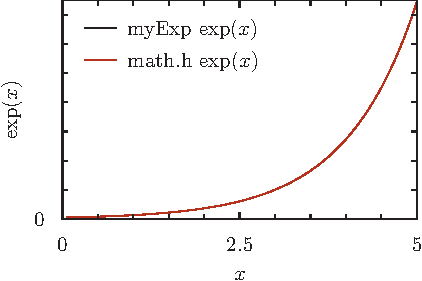
\includegraphics{myExpFunc-fig-pyxplot.pdf}
	\caption{ Plot of numerical implementation as described above, versus the standard implementation found in the header math.h. Notice the two graphs are indistinguishable to the naked eye.}
	\label{fig:pyxplot}
\end{figure}


\end{document}

